\chapter{Algoritmi}

\section{Automatic-ABF} \label{sec:aabf}

\subsection{Introduzione}
La parametrizzazione definisce una corrispondenza tra la mesh 3D e un dominio 2D chiamato spazio di parametrizzazione. L'associazione generata dalla parametrizzazione dovrebbe
assicurare una corrispondenza biunivoca tra i due insiemi. Nelle applicazioni pratiche garantire la corrispondenza biunivoca locale � sufficiente, questo si ottiene se nello
spazio di parametrizzazione non sono presenti triangoli sovvrapposti.

I principali usi della parametrizzazione sono il texture mapping e il geometry editing. Per queste applicazioni la qualit� del risultato dipende fortemente dall'ammontare
delle deformazioni causate dalla parametrizzazione. Idealmente, durante la mappatura, si dovrebbero presevare le aree e gli angoli di tutte le facce ottenendo cos� una
trasformazione isometrica tra i due spazi. Solamente la classe delle superfici sviluppabili ammette una parametrizzazione isometrica, quindi nella pratica sono usati metodi
di parametrizzazione che si basano sulla minimizzazione della distorsione della parametrizzazione.

\subsection{ABF}
Il metodo ABF (angle based flatteling) si basa sull'osservazione che l'insieme degli angoli di una superficie 2D triangolarizzata la definisce univocamente (ad eccezione di
possibili scalamenti e trasformazioni rigide). La procedura utilizzata dall'ABF per prima cosa determina la parametrizzazione nello spazio degli angoli, successivamente
ricava le coordinate 2D. La formulazione del metodo lo porta ad essere particolarmente adatto per ridurre la distorsione angolare della mappatura.
%definzione taglio e vertici interni.

\subsubsection{Formulazione}
Il metodo ABF si basa sulla formulazione del problema attraverso un modello di programmazione non lineare. Definisce quindi una funzione obiettivo da minimizzare, insieme
ad una serie di vincoli che la soluzione deve rispettare. Nello spazio degli angoli la funzione obiettivo da minimizzare � semplicemente 
\begin{eqnarray}   E(\alpha) = \sum_{t \in T} { \sum_{k=1}^{3} {\frac{1}{w_k^t}{(\alpha_k^t - \beta_k^t)}^2 }} \end{eqnarray} 
dove $\alpha_k^t$ sono gli angoli planari (le nostre incognite) e $\beta_k^t$ sono gli angoli ottimali (angoli della mesh 3D). L'indice $t$ varia nell'insieme $T$ dei triangoli della mesh, mentre
l'indice $k$ varia sugli angoli di ciascun triangolo. I pesi $w_k^t$ sono impostati al valore $\frac{1}{{b_k^t}^2}$ per riflettere la distorsione relativa, piuttosto che utilizzare la distorsione
assoluta.

L'impostazione del problema di minimizzazione garantisce la biettivit� locale della parametrizzazione grazie ai vincoli imposti. Durante la risoluzione gli angoli vengono scalati
pi� volte per garantire una soluzione che definisca una parametrizzazione planare valida. Lo spazio delle soluzione viene quindi ridotto spazialmente dai seguenti vincoli
sulle variabili
\begin{itemize}
\item 
Validit� triangolare: ogni triangolo della mesh deve rimanere tale durante la parametrizzazione.
$$V_{Tri}(t) = \alpha_1^t + \alpha_2^t + \alpha_3^t=0, \; \forall t \in T$$
\item Planarit�: ogni vertice della mesh interno alla parametrizzazione deve verificare il vincolo di planarit�.
 $$V_{Plan}(v) = \sum_{(t,k) \in v^*} {\alpha_k^t -2\uppi}=0, \; \forall v \in V_{Int} $$
Dove $V_{Int}$ � l'insieme dei vertici interni alla superficie 2D e $v^*$ � il set degli angoli incidenti al vertice $v$.
\item Integrit� delle raggiere: ogni edge condiviso tra due triangoli deve avere la stessa lunghezza.
$$V_{Len}(v) = \prod_{(t,k) \in v^*} {\sin {\alpha_{k+1}^t}} - \prod_{(t,k) \in v^*} {\sin {\alpha_{k-1}^t}}, \; \forall v \in V_{Int}$$
Gli indici $k+1$ e $k-1$, indicano rispettivamente il prossimo e il precedente angolo del triangolo.
\end{itemize}

% \subsubsection{Vincolo di integrit� delle raggiere}

Analizziamo in dettaglio il vincolo di integrit� delle raggiere. Per prima cosa definiamo la raggiera di centro $v$ come l'insieme dei triangoli aventi $v$ come vertice in comune. Il vincolo garantisce che ogni edge condiviso tra due triangoli della raggiera abbia la stessa lunghezza, in caso contrario potrebbe verificarsi una situazione come quella in figura \ref{fig:alg_aabf_whell}. 

\begin{figure}[!htb]
\centering %
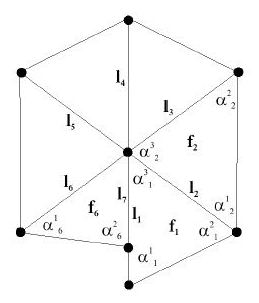
\includegraphics[scale=0.7]{images/algorithms/aabf/whell.jpg}
\caption{raggiera}
\label{fig:alg_aabf_whell}
\end{figure}

Questo vincolo viene espresso in funzione degli angoli esterni della raggiera. Partendo da una coppia di triangoli dobbiamo garantire che l'edge in comune abbia la stessa lunghezza, ci� si pu� esprime come
\begin{eqnarray}  
\frac{l_1}{l_2} = \frac{\sin{\alpha_1^2}}{\sin{\alpha_1^1}}
\end{eqnarray}
procedendo in maniera iterativa lungo la raggiera e in senso antiorario si ottiene
\begin{eqnarray}   
\frac{l_2}{l_3} & = & \frac{\sin{\alpha_2^2}}{\sin{\alpha_2^1}} \\  
\frac{l_1}{l_3} & = & \frac{l_1 l_2}{l_2 l_3} = \frac{\sin{\alpha_1^2}}{\sin{\alpha_1^1}} \cdot \frac{\sin{\alpha_2^2}}{\sin{\alpha_2^1}} \\
\frac{l_1}{l_7} & = & \frac{l_1}{l_2} \cdot \frac{l_2}{l_3} \cdot\cdot\cdot \frac{l_6}{l_7} = \frac{\sin{\alpha_1^2}}{\sin{\alpha_1^1}} \cdot\cdot\cdot \frac{\sin{\alpha_2^2}}{\sin{\alpha_2^1}}  \frac{\sin{\alpha_6^2}}{\sin{\alpha_6^1}}
\end{eqnarray}
Considerando che abbiamo bisogno che $l_7 = l_1$ per ricostruire la raggiera, si ottiene
\begin{eqnarray}   
\frac{\sin{\alpha_1^2}}{\sin{\alpha_1^1}} \cdot\cdot\cdot \frac{\sin{\alpha_2^2}}{\sin{\alpha_2^1}}  \frac{\sin{\alpha_6^2}}{\sin{\alpha_6^1}} = 1
\end{eqnarray}
Una volta fissata la raggiera (e il vertice centrale $v$), il vincolo pu� essere espresso come la differenza di due produttorie. La prima contiene il prodotto dei seni degli angoli destri esterni della raggiera, mentre la seconda il prodotto dei seni degli angoli sinistri esterni della raggiera, in formule
\begin{eqnarray}   
\prod_{\alpha \in A_{estDx}} {\sin {\alpha}} - \prod_{\alpha \in A_{estSx}} {\sin {\alpha}} = 0
\end{eqnarray}
dove $A_{estDx}$ � l'insieme degli angoli esterni destri della raggiera, mentre $A_{estSx}$ � l'insieme degli angoli esterni sinistri della raggiera.

\subsubsection{Meccanismo di risoluzione}
Per la risoluzione del problema abbiamo utilizzato una libreria esterna IpOpt \cite{cit:ipopt}. La libreria implementa una serie di algoritmi per la determinazione di problemi di programmazione non lineare. IpOpt � scritto interamente in C++ e permette di interfacciarsi con altri programma attraverso l'uso e l'estensione di classi. In particolare richiede che il programma client estenda la classe {\scshape TNLP} e che richieda la risoluzione attraverso la classe {\scshape IpoptApplication} caricata da una libreria dinamica esterna.

La classe {\scshape ZedABFProblem} del programma estende le funzionalit� della classe {\scshape TNLP} di IpOpt. Nell'implementazione sono presenti vari metodi richiesti da IpOpt, tra i principali: 
\begin{itemize}
\item 
{\scshape get\_nlp\_info}: questo metodo ritorna alcune informazioni sulla dimensione del problema non lineare, utili alla libreria per allocare sufficiente area di memoria per l'esecuzione;
\item 
{\scshape get\_bounds\_info}: questo metodo definisce per ciascuna variabile il dominio di appartenenza;
\item 
{\scshape get\_starting\_point}: questo metodo assegna un punto di partenza per il problema NLP, viene usato nel caso in cui si utilizzi un'euristica che restituisca una soluzione vicini all'ottimo;
\item 
{\scshape eval\_f}: restituisce il valore della funzione obiettivo nel punto assegnato;
\item 
{\scshape eval\_grad\_f}: restituisce il valore del gradiente della funzione obiettivo nel punto assegnato;
\item 
{\scshape eval\_g}: calcola i valori dei vincoli nel punto assegnato;
\item 
{\scshape eval\_jac\_g}: pu� restituire la struttura della matrice Jacobiana associata ai vincoli, oppure il valore della matrice in un punto dato;
\item 
{\scshape eval\_h}: pu� restituire la struttura della matrice Hessiana della funzione obiettivo, oppure il valore della matrice in un punto dato;
\item 
{\scshape finalize\_solution}: questo metodo � chiamato quando l'algoritmo di ricerca dell'ottimo termina.
\end{itemize}

IpOpt richiede per la risoluzione del problema che sia implementata almeno il metodo {\scshape eval\_grad\_f} che restituisce il valore del gradiente $\bigtriangledown E(\alpha)$. Anche se non strettamente necessario, abbiamo implementato anche il metodo {\scshape eval\_jac\_g} che calcolo il valore della matrice Jacobiana associata ai vincoli del problema, questo permette di velocizzare il processo di risoluzione. In aggiunta era possibile implementare anche il metodo {\scshape eval\_h} per il calcolo della matrice Hessiana della funzione obiettivo.

% Nell'appendice A sono disponbili i codici sorgenti delle funzioni, mentre nell'appendice B sono presenti gli sviluppi matematici per il calcolo del gradiente di $E(\alpha)$ e della matrice Jacobiana, insieme ad altre considerazioni utili.

\subsubsection{Ricostruzione parametrizzazione}
Una volta determinata una soluzione per il problema di minimizzazione � necessario ricostruire la parametrizzazione a partire dagli angoli dello spazio 2D. L'algoritmo di ricostruzione si basa su di un metodo ricorsivo di ricostruzione delle singole raggiere. Per prima cosa fissa un triangolo iniziale da cui partire e successivamente si considera un suo vertice che verr� preso come seme. A partire dal vertice seme si procede con la ricostruzione della raggiera corrispondente, che prevede il calcolo della parametrizzazione di ogni singolo triangolo e la ricorsione su tutti i vertici esterni. Nel listato \ref{alg:abf_reconstruction} � descritto l'algortimo di ricostruzione.

\begin{algorithm}[!htb]
\caption{Algoritmo di ricostruzione}
\label{alg:abf_reconstruction}
\begin{algorithmic}[1]
\Procedure{Parametrizzazione2D} {Geometria G}
	\Require I triangoli di ogni raggiera di G devono essere ordinati in senso anti-orario.
	\State Triangolo t = G.estraiTriangolo(0); 
	\State Vertex seme = e.estraiVertice(0);
	\State Vertex b = e.estraiVertice(1);
	\State seme.inserisciPosizione2D(0, 0);
	\State a.inserisciPosizione2D(0, e.lunghezza());
	\State CostruzioneRaggiera2D(seme);
\EndProcedure
\Statex
\Procedure{CostruzioneRaggiera2D} {Vertice v, Triangolo t, Edge e}
	\State Raggiera R = v.estraiRaggiera();
	\While {t.estraiFlagParametrizzazione() == 0};
		\State ParametrizzaTriangolo(v, t, e);
		\State /* Parametrizza il triangolo t e imposta il suo flag di parametrizzazione a 1 */
		\State 
		\State (t,e) = R.etraiProssimoTriangolo(v, t, e);
		\State /* Estrai il triangolo adiacente a t e l'edge in comune e */
	\EndWhile
	\State
	\For{Vertex i = R.inizioVerticiEsterni(); i != R.fineVerticiEsterni(); i = R.estraiProssimoVertice(i)}
		\State Raggiera nuova\_r = i.estraiRaggiera();
		\State Triangolo prossimo\_t = nuova\_r.estraiPrimoTriangoloLibero();
		\State /* Estrae il primo in senso anti-orario triangolo non marcato con il flag di parametrizzazione. */
		\If{prossimo\_t != NULL}
			\State Triangolo precedente\_t = nuova\_r.estraiTriangoloPrecedente(prossimo\_t);
			\State /* Estrae il triangolo a destra di prossimo\_t all'interno di nuova\_r*/
			\State Edge prossimo\_e = precedente\_t.estraiEdgeComune(prossimo\_t);
			\State CostruzioneRaggiera2D(i, prossimo\_t, prossimo\_e);
		\EndIf
	\EndFor
\EndProcedure
\end{algorithmic}
\end{algorithm}

\subsection{Variazioni sull'ABF}
L'ABF richiede che si definisca l'insieme dei vertici interni nella parametrizzazione, o in modo equivalente l'insieme dei vertici esterni. I vertici esterni definiscono sulla mesh 3D il taglio lungo il quale si effettuer� l'unwrapping della superficie 3D. Per rispettare le specifiche richieste il taglio della mesh non potr� essere definito dall'utente, per questo motivo � necessario definire un metodo di creazione del taglio automatizzato.

Per garantire la capacit� del programma di parametrizzare sempre la mesh utilizzeremo un approccio per la creazione di pi� tagli. Per la determinazione di questi tagli sulla geometria procederemo con un approccio basato sulla visibilit� della geometria da diversi 'punti di vista'. Una volta determinati i tagli otterremmo una serie di sotto-mesh da parametrizzare, per ciascuna di esse utilizzeremo l'ABF per il calcolo della parametrizzazione. Ogni mesh generer� quindi un insieme di sotto-parametrizzazione che andrann� disposte sul piano Ouv della texture.

Descriveremo ora brevemente l'algoritmo per il calcolo dei tagli sulla mesh. Dato un vettore $v$ rappresentante la direzione di visione determiniamo tutti i triangoli che presentano una normale orientata in direzione opposta a $v$. Otterremmo quindi un sotto-superficie della mesh originale, da questa determineremo l'insieme delle superfici completamente collegate da raggiere. A questo punto per ogni sotto-superficie collegata si definisce l'insieme dei vertici esterni, cio� quei vertici tali per cui la raggiera associata non si chiude su se stessa oppure per cui la somma degli angoli interni � maggiore di $2\uppi$. Infine viene determinata la parametrizzazione per ciascuna sotto-superficie collegata, attraverso l'utilizzo del metodo ABF. Il listato \ref{alg:mesh_cut} mostra lo pseudocodice dell'algortimo utilizzato.

\begin{algorithm}[!h]
\caption{Algoritmo di parametrizzazione}
\label{alg:mesh_cut}
\begin{algorithmic}
\Procedure{ParametrizzaGeometria} {Geometria G}
	\State Vector[Vettore] direzioni = calcolaDirezioniOttimali(G);
	\For {Vettore v = direzioni.inizio(); v != direzioni.fine(); v = direzioni.prossimo(v)}
		\State Vector[Triangolo] triangoli = ottieniTriangoliVisibili(G, v);
		\State Vector[Superficie] s\_collegate = calcolaSuperficiColllegate(G, triangoli);
		\For{Superficie s = s\_collgate.inizio(); s != s\_collgate.fine(); s = s\_collgate.prossima(s)}
			\State Vector[Vertice] vertici\_esterni = s.ottieniVerticiEsterni();
			\State G.CollegaSuperficie(S);
			\If{vertici\_esterni.dimensione() != 0}
				\State CalcolaParametrizzazioneABF(G);
			\Else
				\State ImpostaSoluzioneIniziale3D(G);
				\State Parametrizzazione2D(G);
			\EndIf
			\State G.ScollegaSuperficie(S);
		\EndFor
	\EndFor
\EndProcedure
\end{algorithmic}
\end{algorithm}

\section{Greedy packing}

\subsection{Introduzione}
Una volta determinata le parametrizzazione della varie sotto-superfici � necessario disporre le aree ottenute nello spazio $O_{uv}$. L'obiettivo � quello di determinare la disposizione di poligoni all'interno di un quadrato che minimizzi l'ammontare dell'area non utilizzata e nel contempo riduca la dimensione del quadrato necessario a contenerli. La disposizione deve garantire che non siano presenti sovvrapposizioni tra i poligoni (in accordo con la richiesta di biettivit� locale dell'unwrapping).

Il problema di disposizione di oggetti all'interno di uno spazio entra nella categoria dei problemi 'bin packing'. Questa categoria fa' parte dell'insieme dei problemi NP completi, non � quindi possibile determinare un algoritmo che sia in grado di trovare una soluzione ottima al problema. Per questo motivo sono state sviluppate varie euristiche con l'obiettivo di avvicinarsi il pi� possibile alla soluzione al problema.

Per determinare la disposizione dei poligoni all'interno del quadrato abbiamo pensato a realizzare un algoritmo che implementi un approccio greedy al problema. L'obiettivo dell'algoritmo rimane quello di minimizzare l'area inutilizzata all'interno del quadrato, ma per raggiungerlo utilizziamo un approccio differente. Puntiamo infatti a disporre i poligoni in modo da ridurre la crescita del quadrato senza considerazioni particolari sugli spazi non occupati.

\subsection{Algoritmo di packing}
L'algoritmo di packing permette di determinare una disposizione valida delle superfici bidimensionali nello spazio $O_{uv}$. Non garantisce di determinare la disposizione ottima secondo una particolare metrica, ma affronta il problema utilizzando un approccio greedy. L'algoritmo di packing � implementata nella classe {\scshape ZedAOPolygonPacker}, questa agisce su una serie di oggetti del tipo {\scshape ZedAOPolygonPack} che rappresentano le aree bidimensionali da disporre sul piano $O_{uv}$. La classe {\scshape ZedAOPolygonPacker}  implementa un meccanismo di creazione di bordi intorno alle superfici 2D per permettere di eliminare alcuni fenomeni di discontinuit� che si venivano a creare sulla mesh con applicata la texture.

Descriviamo ora il procedimento utilizzato per il packing delle superfici bidimensionali ottenute dalla parametrizzazione. Per prima cosa ogni parametrizzazione della mesh ottenuta dall'esecuzione dell'A-ABF viene convertita in un poligono convesso per il packing. Viene creato un vettore di istanze della classe {\scshape ZedAOPolygonPack}, questa implementa varie funzionalit� sulle superfici tra cui il calcolo del convex hull per determinare il poligono convesso dati una serie di vertici (nell'appendice viene trattato nei dettagli).

Si prosegue con il calcolo della disposizione. Il vettore dei poligoni viene ordinato per valore di area decrescente, quindi per ciascuno viene determinata la disposizione ottimale con la configurazione fino a quel momento ottenuta. La disposizione iniziale si ottiene dal primo poligono della lista, si prosegue determinando la posizione ottimale del primo poligono in lista, lo si estra e lo si aggiunge alla configurazione attuale, quindi si riesegue fino a quando la lista non � vuota.

Il calcolo della disposizione ottimale del poligono dato all'interno del quadrato si compone di due fasi. Nella prima fase si determina la regione di movimento del poligono, cio� dove il poligono pu� muoversi. Nella seconda fase si determina qual'� la disposizione del poligono che minimizza la dimensione del quadrato che contiene il poligono e la configurazione precedente.

Dopo aver determinato il poligono di non sovvraposizione viene calcolata la posizione di $Q$ che minimizza la dimensione del quadrato che inscrive i poligoni. Il poligono $Q$ viene traslato in ogni punto di $PQ$ e per ogni posizione viene calcolata l'area del quadrato, alla fine si sceglie la posizione con area minima e si trasla $Q$ nel punto. Q viene quindi inclusa nella soluzione attuale e si procede con il prossimo poligono da disporre.

\subsection{Dettagli sul calcolo della regione di non sovrapposizione}
L'algoritmo per il calcolo della regione di movimento si basa sul lavoro presente in \cite{cit:nofit}. La procedura da loro ideata permette di determinare il poligono di non sovrapposizione a partire da due poligoni (non necessariamente convessi). Questo viene calcolato a partire da due poligoni, uno fisso e l'altro orbitante intorno al pirmo; consente la definzione della frontiera che divide il piano in due regioni, una in cui il poligono orbitante � libero di muoversi e l'altra non accessibile (per evitare sovvrapposizioni).

Dato un sistema di riferimento cartesiano $O_{xy}$, l'algoritmo considera uno dei due poligoni come fissato e l'altro libero di muoversi. Da ora in poi chiameremo $P$ il poligono fisso in $O_{xy}$ mentre $Q$ quello libero e $PQ$ il poligono di non sovrapposzione. Per calcolare i vertici del poligono $PQ$ l'algoritmo procede per traslazioni successive eseguite su $Q$ (un suo vertice viene preso come riferimento per delineare il profilo di $PQ$). L'algortimo calcola per prima cosa tutte le coppie di edge di $P$ e $Q$ che si incontrano almeno per un punto, tra questi si scelgono un insieme di edge che potranno essere usato come vettori di traslazione. Tra i possibili edge candidati a diventare il vettore di traslazione vengono scelti solo quelli che non provocano sovvrapposizione tra $P$ e $Q$. Viene quindi scelto il vettore per la traslazione di $Q$, nel caso in cui $Q$ sia tornato nella posizione originale l'esecuzione termina altrimenti si ricominicia.

